\documentclass[]{article}
\usepackage[top=1.3in,bottom=1.3in,left=1in,right=1in]{geometry}
\usepackage{tikz}
\usetikzlibrary{shapes.geometric,arrows.meta}
\usepackage{subcaption}
\usepackage{xcolor}
\usepackage[colorlinks,allcolors=blue]{hyperref}
\usepackage[noabbrev]{cleveref}

\usepackage{xcolor}

\title{
    {\LARGE Project Part A}
    \\[1ex]
    {\Huge\bf Searching}
}
\author{
    COMP30024 Artificial Intelligence
}
\date{2021}


% Custom TikZ commands
\newcommand{\hex}[4] {
    \node[hex,fill={#3}] at ({#1}, {#2}) {};
    \node[hex,thick,draw={#3},fill={#3!10}] at ({#1}, {#2}) {};
    \node at ({#1}, {#2}) {{#4}};
}
\newcommand{\uptoken}[4] {
    \node[draw,circle,minimum size=4.5mm,fill=white] (#4) at (#1, #2) {};
    \node[draw,circle,minimum size=3.7mm,very thick,black]  at (#1, #2) {};
    \node[] at (#1, #2) {#3};
}
\newcommand{\lotoken}[4] {
    \node[draw,circle,minimum size=4.5mm,fill=white] (#4) at (#1, #2) {};
    \node[draw,circle,minimum size=3.7mm,very thick,purple] at (#1, #2) {};
    \node[] at (#1, #2) {#3};
}

\newcommand{\board} {
    \tikzset{
        hex/.style={
            regular polygon,
            regular polygon sides=6,
            minimum size=10mm,
            inner sep=0mm,
            outer sep=0mm,
            rotate=30,
            draw
        },
        x={(4.33mm,7.5mm)},
        y={(8.66mm,0mm)}
    }
    \foreach \r/\q in {
                    +4/-4,+4/-3,+4/-2,+4/-1,+4/+0,
                 +3/-4,+3/-3,+3/-2,+3/-1,+3/+0,+3/+1,
              +2/-4,+2/-3,+2/-2,+2/-1,+2/+0,+2/+1,+2/+2,
           +1/-4,+1/-3,+1/-2,+1/-1,+1/+0,+1/+1,+1/+2,+1/+3,
        +0/-4,+0/-3,+0/-2,+0/-1,+0/+0,+0/+1,+0/+2,+0/+3,+0/+4,
           -1/-3,-1/-2,-1/-1,-1/+0,-1/+1,-1/+2,-1/+3,-1/+4,
              -2/-2,-2/-1,-2/+0,-2/+1,-2/+2,-2/+3,-2/+4,
                 -3/-1,-3/+0,-3/+1,-3/+2,-3/+3,-3/+4,
                    -4/+0,-4/+1,-4/+2,-4/+3,-4/+4,
    }
        \node[hex,fill=black!5] at (\r, \q) {};
}



\begin{document}

\maketitle


\section*{Overview}

In this first part of the project, we will play a simplified, single-player
(non-adversarial), search-based variant of the game of \emph{RoPaSci~360}.
Before you read this specification, please make sure you have carefully
read the entire `Rules for the Game of \emph{RoPaSci~360}' document.

The aims for Project Part A are for you and your project partner to
(1)~refresh and extend your Python programming skills,
(2)~explore some of the algorithms you have met in lectures, and
(3)~become more familiar with some core mechanics of \emph{RoPaSci~360}.
%
This is also a chance for you to develop fundamental Python tools for
working with the game:
Some of the functions and classes you create now may be helpful later
(when you are building your full game-playing program for Part B of
the project).


\subsection*{Single-player \emph{RoPaSci~360}}

The single-player game we will analyse is based on \emph{RoPaSci~360},
with the following modifications:
%
\begin{enumerate}
    \item
        There is \emph{no throw action}. Instead, the game begins with
        tokens already on the board.
    \item
        Lower's tokens \emph{never move.}
        On each turn, \emph{all} of Upper's tokens move (each using a
        \emph{slide} or \emph{swing} action), all at the same time.
        If Upper has more than one token, they all move at the same time.
    \item
        The player must repeatedly move the Upper tokens to \emph{defeat
        all of Lower's tokens} to win.
        If the last Upper token is defeated in the same turn as the last
        Lower token, the player still wins.
    \item
        There is a new type of token:
        \textbf{Block tokens} prevent other tokens from occupying their
        hexes. Block tokens never move. No token can slide or swing onto
        or over a Block token.
\end{enumerate}
%
Most of the other rules (for example, the rules for slide and swing actions,
and the rules for token battles on shared hexes and defeating tokens) are
the same as in the original \emph{RoPaSci~360} game.


\subsection*{The tasks}

Firstly, you will \textbf{design and implement a program} that `plays' a
game of single-player \emph{RoPaSci~360}.
That is, given a starting board configuration, the program must find a
sequence of actions to win the game (to defeat all Lower tokens).
Secondly, you will \textbf{write a brief report} discussing and analysing
the strategy your program uses to solve this search problem.
These tasks are described in detail in the following sections.


\section*{The program}

You must create a program to play this game in the form of a Python 3.6
\textbf{module}\footnotemark\ called \texttt{search}.

\footnotetext{
    This module might be a \emph{single file} called \texttt{search.py}, or
    it might include multiple files in a directory called \texttt{search/},
    with an entry-point in \texttt{search/\_\_main\_\_.py}. Either way, you
    should be able to run the program using the command
    \texttt{python~-m~search} (followed by command-line arguments).
    See the skeleton code for an example of the correct structure.
}

When executed, your program must read a JSON-formatted board
configuration from a file, calculate a winning sequence of actions, and
print out this sequence of actions.
%
The input and output format are specified below, along with the coordinate
system we will use for both input and output.


\subsection*{Coordinate system}

For input and output, we'll index the board's hexes with an
\emph{axial coordinate system}\footnotemark.
In this system each hex is addressed by a \textbf{row} ($r$) and
\textbf{column} ($q$) pair, as shown in \Cref{fig:coordinates}.

\begin{figure}[ht!]
    \centering
    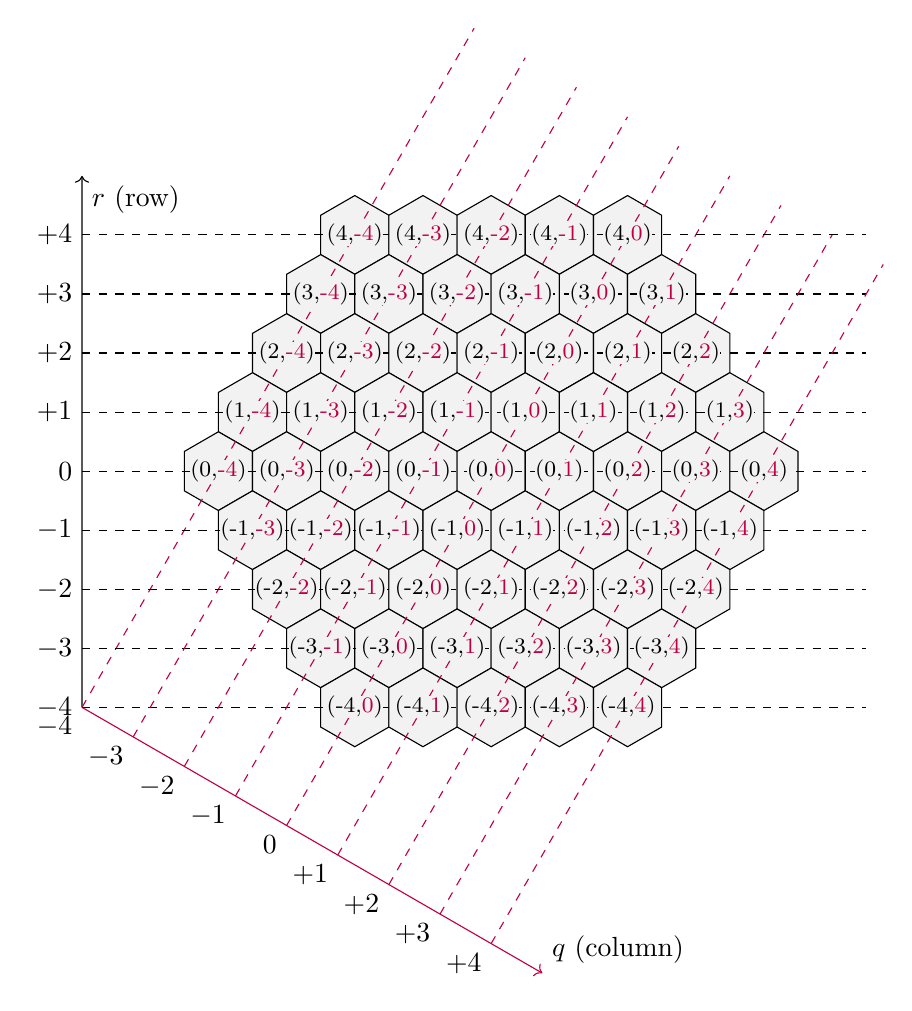
\begin{tikzpicture}
        % \clip (-6, -6.4) rectangle (5, 4);
        \board
        % draw r axis
        \draw (-4, -4) edge[->] (5, -8.5);
        \node[below right] at (5, -8.5)  {$r$ (row)};
        % draw q axis
        \draw (-4, -4) edge[->,purple] (-8.5, 5);
        \node[above right] at (-8.5, 5) {$q$ (column)};
        % draw dashed grid
        \foreach \i/\j in {0/-4,1/-3,2/-2,3/-1,4/0,5/+1,6/+2,7/+3,8/+4} {
            \node[left] at (\j, -4-0.5*\i) {$\j$};
            \draw (\j,-4-0.5*\i) edge[dashed] (\j,7.5-0.5*\i);
            \node[below left] at (-4-0.5*\i, \j) {$\j$};
            \draw (-4-0.5*\i,\j) edge[dashed,draw=purple] (7.5-0.5*\i,\j);
        }
        % draw all points
        \foreach \r/\q in {4/-4,4/-3,4/-2,4/-1,4/0,3/-4,3/-3,3/-2,3/-1,3/0,
            3/1,2/-4,2/-3,2/-2,2/-1,2/0,2/1,2/2,1/-4,1/-3,1/-2,1/-1,1/0,1/1,
            1/2,1/3,0/-4,0/-3,0/-2,0/-1,0/0,0/1,0/2,0/3,0/4,-1/-3,-1/-2,
            -1/-1,-1/0,-1/1,-1/2,-1/3,-1/4,-2/-2,-2/-1,-2/0,-2/1,-2/2,-2/3,
            -2/4,-3/-1,-3/0,-3/1,-3/2,-3/3,-3/4,-4/0,-4/1,-4/2,-4/3,-4/4}
            \node[fill=black!5,inner sep=0pt] at (\r,\q)
                {\footnotesize (\r,{\color{purple}\q})};
    \end{tikzpicture}
    \caption{\label{fig:coordinates}
        The $r$ and $q$ axes, with $(r, q)$ indices for all hexes.
    }
\end{figure}

\footnotetext{
    The following guide to hexagonal grids may prove useful:
    \href
        {https://redblobgames.com/grids/hexagons}
        {\tt redblobgames.com/grids/hexagons/}.
    %
    In particular, see the `coordinates' section for notes on a
    similar axial coordinates system.
    %
    \textbf{Don't forget to acknowledge} any algorithms or code you
    use in your program.
}


\subsection*{Input format}

Your program must read a board configuration from a JSON-formatted file.
The name of the file will be given to your program as its first and only
command-line argument.\footnotemark\ 
The JSON file will contain a single dictionary (JSON object) with the
following three entries:
%
\begin{itemize}
    \item
        An entry with key \texttt{"upper"} specifying the starting position
        of Upper's tokens as a list of token descriptions
        (as described below).
    \item
        An entry with key \texttt{"lower"} specifying the position
        of Lower's tokens as a list of token descriptions.
    \item
        An entry with key \texttt{"block"} specifying the position of any
        blocking tokens as a list of token descriptions.
\end{itemize}
%        
Each token description is a list of the form
\texttt{{[}$s$,$r$,$q${]}} where
$s$ is a string representing the token's symbol
(\texttt{"r"} for Rock, \texttt{"p"} for Paper, \texttt{"s"} for Scissors;
blocking tokens have no symbol and use the string \texttt{""}),
%
and $(r, q)$ are the axial coordinates of the token's hex
(see \Cref{fig:coordinates}).

\footnotetext{
    We recommended using Python's Standard Library module `\texttt{json}'
    for loading this input.
    An appropriate call would be
    `\texttt{with open{(}sys.argv{[}1{]}{)} as file: data = json.load(file)}'
    (creating \texttt{data}, a dictionary version of the input).
}

You may assume that
(1) the input matches this format description exactly
(we will not give you invalid JSON),
(2) all token descriptions contain valid coordinates
(we will not give you coordinates outside of the board),
(3) there are no overlapping tokens
(we will not give you a configuration with two tokens initially on the same
hex), and
(4) there is at least one winning sequence of actions
(we will not give you configurations from which it is impossible to win).

\subsection*{Output format}

Your program must print out the actions Upper should take on each turn to
win the game.
The actions must be printed to \emph{standard output}\footnotemark,
with one line of output per action, in the following format:
%
\begin{itemize}
    \item
        To output a slide action on turn $t$ for a token on hex $(r_a, q_a)$
        sliding to hex $(r_b, q_b)$, print the line:
    `\texttt{Turn~$t$:\ SLIDE\ from\ ($r_a$,$q_a$)\ to\ ($r_b$,$q_b$)}'.
    \item
        To output a swing action on turn $t$ for a token on hex $(r_a, q_a)$
        swinging to hex $(r_b, q_b)$, print the line:
    `\texttt{Turn~$t$:\ SWING\ from\ ($r_a$,$q_a$)\ to\ ($r_b$,$q_b$)}'.
\end{itemize}
%
The first turn is numbered 1, and note that in this single-player variant of
the game, Upper will take \emph{one action with each token on each turn}, and
these actions happen at the same time.
For example, if Upper controls three tokens, the first three lines of output
should all begin with `\texttt{Turn 1:}'.

\footnotetext{
    Your program \emph{should not print any other lines to standard output}.
    However, we will ignore lines beginning with the character `\texttt{\#}',
    so you may use this character to begin any lines of output that are not
    part of your action sequence.
}

\begin{figure}[ht!]
\centering
\begin{subfigure}[b]{.28\textwidth}
\centering
\begin{verbatim}
{
  "upper": [["s", 2,-1],
            ["r",-3, 2]],
  "lower": [["s", 1,-1],
            ["p",-1, 1]],
  "block": [["",  0, 0]]
}
\end{verbatim}
\caption{\label{fig:eginput}
    An example input file.
}
\end{subfigure}
\begin{subfigure}[b]{.30\textwidth}
\centering
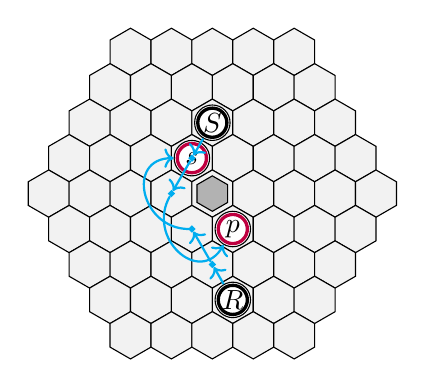
\begin{tikzpicture}
    \tikzset{
        hex/.style={regular polygon,regular polygon sides=6,minimum size=6mm,
            inner sep=0mm,outer sep=0mm,rotate=30,draw},
        x={(2.598mm,4.5mm)},y={(5.196mm,0mm)}
    }
    \foreach \r/\q in {+4/-4,+4/-3,+4/-2,+4/-1,+4/+0,+3/-4,+3/-3,+3/-2,+3/-1,
           +3/+0,+3/+1,+2/-4,+2/-3,+2/-2,+2/-1,+2/+0,+2/+1,+2/+2,+1/-4,+1/-3,
           +1/-2,+1/-1,+1/+0,+1/+1,+1/+2,+1/+3,+0/-4,+0/-3,+0/-2,+0/-1,+0/+0,
           +0/+1,+0/+2,+0/+3,+0/+4,-1/-3,-1/-2,-1/-1,-1/+0,-1/+1,-1/+2,-1/+3,
           -1/+4,-2/-2,-2/-1,-2/+0,-2/+1,-2/+2,-2/+3,-2/+4,-3/-1,-3/+0,-3/+1,
           -3/+2,-3/+3,-3/+4,-4/+0,-4/+1,-4/+2,-4/+3,-4/+4}
        \node[hex,fill=black!5] at (\r, \q) {};
    % block
    \node[hex,minimum size=4.5mm,fill=black!30] at (0,0) {};
    % tokens
    \uptoken{-3}{+2}{$R$}{1}
    \uptoken{+2}{-1}{$S$}{2}
    \lotoken{-1}{+1}{$p$}{3}
    \lotoken{+1}{-1}{$s$}{4}
    % steps
    \begin{scope}[draw=cyan]
        \node[inner sep=0pt,draw,circle,very thick] (s0) at (-2,+1) {};
        \node[inner sep=0pt,draw,circle,very thick] (s1) at (-1,+0) {};
        \node[inner sep=0pt,draw,circle,very thick] (s2) at (+1,-1) {};
        \node[inner sep=0pt,draw,circle,very thick] (s3) at (+0,-1) {};
        \draw[thick,->] (1)  -- (s0);
        \draw[thick,->] (s0) -- (s1);
        \draw[thick,->] (s1) edge[out=180,in=180,looseness=1.7] (4);
        \draw[thick,->] (2)  -- (s2);
        \draw[thick,->] (s2) -- (s3);
        \draw[thick,->] (s3) edge[out=240,in=240,looseness=1.7] (3);
    \end{scope}
\end{tikzpicture}
\caption{\label{fig:egboard}
    Starting board and a solution.
}
\end{subfigure}
\begin{subfigure}[b]{.40\textwidth}
\centering
\begin{verbatim}
# Lines like this are ignored
Turn 1: SLIDE from (2,-1) to (1,-1)
Turn 1: SLIDE from (-3,2) to (-2,1)
# Both Scissors now share a hex
Turn 2: SLIDE from (1,-1) to (0,-1)
Turn 2: SLIDE from (-2,1) to (-1,0)
# Note, turn happens all at once:
Turn 3: SWING from (0,-1) to (-1,1)
Turn 3: SWING from (-1,0) to (1,-1)
\end{verbatim}
\caption{\label{fig:egoutput}
    Standard output for this solution.
}
\end{subfigure}
\end{figure}


\section*{The report}

Finally, you must briefly discuss your approach to solving this problem
in a separate file called \texttt{report.pdf} (to be submitted alongside
your program). Your discussion should answer these three questions:
%
\begin{enumerate}
    \item
        How did you formulate this game as a search problem?
        Explain your view of the problem in terms of states, actions, goal
        tests, and path costs, as relevant.
    \item
        What search algorithm does your program use to solve this problem,
        and why did you choose this algorithm?
        Comment on the algorithm's efficiency, completeness, and optimality.
        If you have developed heuristics to inform your search, explain them
        and comment on their admissibility.
    \item
        How do the features of the starting configuration (the position and
        number of tokens) impact your program's time and space requirements?
        For example, discuss their connection with the branching factor and
        search tree depth and how these affect the time and space complexity
        of your algorithm.
\end{enumerate}
%
Your report can be written using any means but must be submitted as
\textbf{a PDF document}.
Your report should be between 0.5 and 2 pages in length, and must not
be longer than 2 pages (excluding references, if any).


\section*{Assessment}

Your team's Project Part A submission will be assessed out of 8~marks,
and contribute 8\% to your final score for the subject.
Of these 8~marks:

\begin{itemize}
    \item
        \textbf{5 marks} will be for the correctness of your program.
        based on running your program through a collection of automated
        test cases of increasing complexity, as described below.
        %
        The first mark is earned by correctly following the input and
        output format requirements.
        % 
        The remaining four marks are available for passing the tests at
        each of the following four difficulty `levels':\footnotemark
        \footnotetext{
            It may help to break this task down into stages.
            For example, begin by implementing a program that can pass
            tests of `difficulty level 1', then move on to the higher
            levels.
            %
            Furthermore, even if you don't have a program that works
            correctly by the time of the deadline, you may be awarded
            some marks for making a reasonable attempt.
        }
        % 
        \begin{enumerate}
            \item
                Upper and Lower each begin with a single token. There are no
                blocking tokens.
            \item
                Upper begins with 1 token and Lower begins with 2--9 tokens.
                There may be blocking tokens.
            \item
                Upper begins with 2 tokens and Lower begins with 1--9 tokens.
                There may be blocking tokens.
            \item
                Upper begins with 3 tokens and Lower begins with 1--9 tokens.
                There may be blocking tokens.
        \end{enumerate}
        %
        The tests will run with \textbf{Python 3.6} on the \textbf{student
        Unix machines} (for example, \texttt{dimefox}\footnotemark).
        \footnotetext{
            We strongly recommended that you test your program on
            \texttt{dimefox} before submission. Seek our help early if
            you cannot access \texttt{dimefox}.
            %
            Note that Python 3.6 is not available on \texttt{dimefox} by
            default, but it can be used after running the command
            `\texttt{enable-python3}' (once per login).
        }
        %
        There will be a \textbf{30 seconds time limit} per test case.
        Programs that do not run in this environment or do not complete
        within this time will be considered incorrect.
    \item
        \textbf{3 marks} will be for the clarity and accuracy of the
        discussion in your \texttt{report.pdf} file, with 1~mark allocated
        to each of the three questions listed above.
        A mark will be deducted if the report is longer than 2~pages or not a
        PDF document.
\end{itemize}

Your program should use \textbf{only standard Python libraries}, plus the
optional third-party libraries \textbf{NumPy and SciPy}
(these are the only libraries installed on \texttt{dimefox}).
%
With acknowledgement, you may also include code from the AIMA textbook's
Python library, where it is compatible with Python 3.6 and the above
limited dependencies.



\subsection*{Academic integrity}

Unfortunately, we regularly detect and investigate potential academic
misconduct and sometimes this leads to formal disciplinary action from
the university.
%
Below are some guidelines on academic integrity for this project.
%
Please refer to the university's academic integrity website
(\href{https://academicintegrity.unimelb.edu.au}{\texttt{academicintegrity.unimelb.edu.au}})
or ask the teaching team,
if you need further clarification.

\begin{enumerate}
    \item
        You are encouraged to discuss ideas with your fellow students, but
        \textbf{it is not acceptable to share code between teams, nor to
        use code written by anyone else}.
        %
        Do not show your code to another team or ask to see another team's
        code.
    \item
        You are encouraged to use code-sharing/collaboration services,
        such as GitHub, \emph{within} your team.
        %
        However, \textbf{you must ensure that your code is never visible
        to students outside your team}.
        %
        Set your online repository to `private' mode, so that only your
        team members can access it.
    \item
        You are encouraged to study additional resources to improve your
        Python skills.
        %
        However, \textbf{any code adapted or included from an external
        source must be clearly acknowledged}.
        %
        If you use code from a website, you should include a link to the
        source alongside the code.
        %
        When you submit your assignment, you are claiming that the work
        is your own, except where explicitly acknowledged.
\end{enumerate}


\section*{Submission}

One submission is required from each team. That is, one team member is
responsible for submitting all of the necessary files that make up your
team's solution.

You must submit a single compressed archive file (e.g.~a \texttt{.zip}
or \texttt{.tar.gz} file) containing all files making up your solution
via the `Project Part A Submission' item in the `Assessments' section of
the LMS. This compressed file should contain all Python files required
to run your program, along with your report.

\begin{center}
    The submission deadline is
    \textbf{11:00PM on Wednesday the 31\textsuperscript{st} March,
    Melbourne time (AEDT).}
\end{center}

You may submit multiple times.
%
We will mark the latest submission made by either member of your
team unless we are advised otherwise.
%
You may submit late.
%
Late submissions will incur a penalty of \textbf{one mark per working day}
(or part thereof) late.

\subsection*{Extensions}

If you require an extension, please email the lecturers using the
subject `COMP30024 Extension Request' at the earliest possible
opportunity.
%
If you have a medical reason for your request, you will be asked to
provide a medical certificate.
%
Requests for extensions received after the deadline may be declined.

\end{document}
